\documentclass[a4paper,12pt,justified,twoside,notoc]{tufte-book}

%% Well understand input, and nice output
\usepackage[utf8]{inputenc}
\usepackage{lmodern}
\usepackage[T1]{fontenc}
\usepackage[french]{babel}

\hypersetup{colorlinks}  % uncomment this line if you prefer colored hyperlinks (e.g., for onscreen viewing)

%% Book metadata
\title{``Chasse aux trésors photographique \\ au Musée du Louvre''}
\author[Lilian \& Hélène]{Lilian Besson \& Hélène Javelaud}
\publisher{``À nos 50 ans'', samedi 10 février 2018}

\usepackage{palatino}

%% For nicely typeset tabular material
\usepackage{booktabs}

%% For graphics / images
\usepackage{graphicx}
\setkeys{Gin}{width=\linewidth,totalheight=\textheight,keepaspectratio}
\graphicspath{{pictures/}}

% The fancyvrb package lets us customize the formatting of verbatim
% environments.  We use a slightly smaller font.
\usepackage{fancyvrb}
\fvset{fontsize=\normalsize}

%% Prints a trailing space in a smart way.
\usepackage{xspace}

%% https://tex.stackexchange.com/a/157404/
\usepackage[tocflat]{tocstyle}
\usetocstyle{standard}


%% Prints the month name (e.g., January) and the year (e.g., 2008)
\newcommand{\monthyear}{%
  \ifcase\month\or janvier\or février\or mars\or avril\or mai\or juin\or
  juillet\or août\or septembre\or octobre\or novembre\or
  décembre\fi\space\number\year
}

\providecommand{\tightlist}{%
\setlength{\itemsep}{0pt}\setlength{\parskip}{0pt}}

% Inserts a blank page
\newcommand{\blankpage}{\newpage\hbox{}\thispagestyle{empty}\newpage}

% Define macros for config
% This is automatically generated with 'prebuild.sh', DO NOT EDIT BY HAND.
\newcommand{\nbequipes}{2}
\newcommand{\nbparequipe}{4}
\newcommand{\totalnbenigmes}{50}
\newcommand{\nbenigmes}{25}


\global\marginparsep=34pt
\global\marginparwidth=124pt
\global\textwidth=285pt
% \global\inner=1cm
% \global\outer=2cm

\begin{document}


% r.3 full title page
\maketitle


% v.4 copyright page
\newpage
\begin{fullwidth}

\begin{center}
  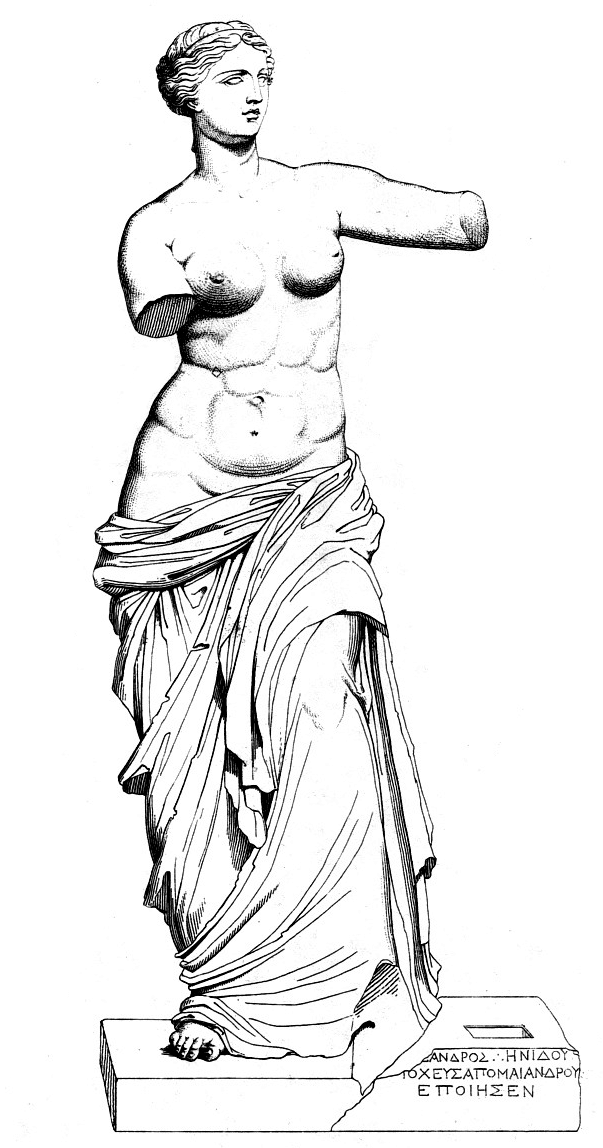
\includegraphics[width=0.70\textwidth]{Paris_Louvre_Venus_de_Milo_Debay_drawing.png}
\end{center}

~
\vfill
\thispagestyle{empty}
\setlength{\parindent}{0pt}
\setlength{\parskip}{\baselineskip}
Copyright \copyright\ \the\year\ \thanklessauthor

% \par\smallcaps{https://github.com/Naereen/Chasse-aux-tr-sors-au-Louvre-pour-mes-25-ans}

\par Cette œuvre est mise à disposition sous licence Attribution - Pas d'Utilisation Commerciale - Pas de Modification 4.0 International. Pour voir une copie de cette licence, visitez \url{http://creativecommons.org/licenses/by-nc-nd/4.0/} ou écrivez à Creative Commons, PO Box 1866, Mountain View, CA 94042, USA.\index{license}

\par\textit{Première édition, \monthyear}.
\end{fullwidth}

% r.5 contents
\setcounter{tocdepth}{2}

\begin{large}
  \tableofcontents
\end{large}

% \listoffigures
% \listoftables

% ---

% r.9 introduction
\cleardoublepage
\chapter{Introduction}

\vspace*{-30pt}

Chères amies et chers amis, merci d'avoir répondu présent !
%
Vous voilà réunis par \textbf{équipe de \intervalparequipe{} personnes},
et vous avez \textbf{\nbenigmes{} tâches à effectuer}.
%
Vous avez \textbf{maximum $3$ heures} : le musée évacue à \textbf{17h45} !
%
Rendez-vous sous l'Arc de Triomphe du Carrousel, \textbf{à 18h.}
% la statue ``Retour de chasse''\footnote{Préparez-vous, les jeux de mots et clins d'œil sont nombreux !}
% Retour de chasse, Antonin Carlès (1888 ; 48° 51′ 49″ N, 2° 19′ 53″ E)
% https://fr.wikipedia.org/wiki/Liste_des_%C5%93uvres_publiques_du_1er_arrondissement_de_Paris#Jardins_des_Tuileries


\section*{Règle du jeu}

L'ordre des énigmes est \emph{aléatoire}, elles ne sont triées ni par ordre chronologique, ni logique, ni spatial dans le musée, et n'ont aucune dépendance entres elles.
%
Toutes peuvent être résolues sans enfreindre le règlement intérieur du musée.
% il n'y a aucun piège.
Munissez vous d'un appareil photo ou de vos \emph{smartphones} : \textbf{toutes les énigmes demandent de trouver une œuvre et de la prendre en photo}\footnote{Sans flash ! Pas de retouchage des photos, non plus !}. SVP, pensez bien à photographier aussi les étiquettes des œuvres !
Et si vous pouviz aussi noter le numéro de la salle de votre trouvaille, pour chaque énigme, directement sur le livret, ce serait chouette\footnote{On fera un joli petit site Internet qui montrera vos solutions pour chaque énigmes, avec leur localisation dans le musée} !
\textbf{Pas de triche} : n'utilisez pas vos smartphones pour chercher sur Internet !
Économisez votre batterie et relayez vous.
%
Vous êtes réunis dans une équipe homogène, donc pensez à mobilisez les idées et connaissances\footnote{Je n'ai pas pu m'empêcher de glisser quelques calculs mathématiques… -- Lilian} de tout le monde (et faites connaissance) !

Tâchez d'être l'équipe la plus rapide ! La coopération entre les autres équipes n'est pas interdite…
Mais vous n'avez pas les mêmes énigmes qu'eux, et la meilleure équipe recevra un prix ce soir !
%
Un dernier conseil : restez calmes et discrets… il ne faut pas que les vigiles détectent que vous vous êtes lancés dans une chasse aux trésors…


\section*{Bonne chance !}
Affûtez votre regard, aiguisez votre attention, entrez dans le Musée du Louvre, et vous voilà près à affronter les autres équipes !



% r.10 all the enigmas
\cleardoublepage
\chapter{Énigmes}

\begin{fullwidth}
% This is automatically generated with 'build.sh', DO NOT EDIT BY HAND.
\input{./src/48.tex}
\input{./src/49.tex}
\input{./src/12.tex}
\input{./src/20.tex}
\input{./src/3.tex}
\input{./src/13.tex}
\input{./src/16.tex}
\input{./src/43.tex}
\input{./src/37.tex}
\input{./src/15.tex}
\input{./src/22.tex}
\input{./src/36.tex}
\input{./src/41.tex}
\input{./src/5.tex}
\input{./src/39.tex}
\input{./src/9.tex}
\input{./src/6.tex}
\input{./src/4.tex}
\input{./src/25.tex}
\input{./src/24.tex}
\input{./src/33.tex}
\input{./src/26.tex}
\input{./src/34.tex}
\input{./src/40.tex}
\input{./src/30.tex}

\end{fullwidth}


% r.10 conclusion
\cleardoublepage
\chapter{À propos}

\section*{Un petit mot des créateurs}

Nous espérons que ce livret et ce moment vont vous plaire !
On s'est bien amusé à le concevoir, c'est déjà ça...

Si un problème survient, ou que vous bloquez sur une énigme, que vous pensez avoir besoin d'aide\footnote{Par exemple si vous pensez qu'une erreur s'est glissée dans ce document…}, n'hésitez pas à nous contacter par téléphone ou nous appeler
\input{telephones.tex}.

Nous avons hâte de vous retrouver dans le jardin des tuileries afin de décerner le \emph{prix de la meilleure équipe !}
Toutes les équipes auront une récompense, ne vous inquiétez pas…


\section*{Aspect ``technique'' \& remarques geek}
Ce document a été rédigé et compilé par mes soins (Lilian), en sélectionnant \emph{aléatoirement} \nbenigmes{} énigmes parmi une liste plus grande\footnote{\url{Goo.gl/JmPFeb}} de \totalnbenigmes{} énigmes.
%
Chaque énigme a été rédigée comme un petit document Markdown\footnote{\url{DaringFireball.net/projects/markdown/}},
qui est ensuite compilé en \LaTeX{} par \texttt{pandoc}\footnote{\url{pandoc.org/}}.
%
Le document principal est un simple document \LaTeX,
utilisant le style épuré de Tufte-\LaTeX{}\footnote{\url{GitHub.com/Tufte-LaTeX/tufte-latex}}.
%
Les sources sont en accès libre\footnote{\url{Goo.gl/eM6wcj}} et sous licence Creative Commons.

Ce recueil à été rédigé, imprimé et relié avec amour en janvier et février 2018.


\hfill{} -- \emph{Lilian Besson \& Hélène Javelaud}.

\section*{Remarque importante}
Aucun bénéfice financier n'a été ni ne sera tiré de ce document.
C'est juste pour s'amuser !


\newpage
\blankpage

\end{document}
